% Template for PLoS
% Version 3.3 June 2016
%
% % % % % % % % % % % % % % % % % % % % % %
%
% -- IMPORTANT NOTE
%
% This template contains comments intended 
% to minimize problems and delays during our production 
% process. Please follow the template instructions
% whenever possible.
%
% % % % % % % % % % % % % % % % % % % % % % % 
%
% Once your paper is accepted for publication, 
% PLEASE REMOVE ALL TRACKED CHANGES in this file 
% and leave only the final text of your manuscript. 
% PLOS recommends the use of latexdiff to track changes during review, as this will help to maintain a clean tex file.
% Visit https://www.ctan.org/pkg/latexdiff?lang=en for info or contact us at latex@plos.org.
%
%
% There are no restrictions on package use within the LaTeX files except that 
% no packages listed in the template may be deleted.
%
% Please do not include colors or graphics in the text.
%
% The manuscript LaTeX source should be contained within a single file (do not use \input, \externaldocument, or similar commands).
%
% % % % % % % % % % % % % % % % % % % % % % %
%
% -- FIGURES AND TABLES
%
% Please include tables/figure captions directly after the paragraph where they are first cited in the text.
%
% DO NOT INCLUDE GRAPHICS IN YOUR MANUSCRIPT
% - Figures should be uploaded separately from your manuscript file. 
% - Figures generated using LaTeX should be extracted and removed from the PDF before submission. 
% - Figures containing multiple panels/subfigures must be combined into one image file before submission.
% For figure citations, please use "Fig" instead of "Figure".
% See http://journals.plos.org/plosone/s/figures for PLOS figure guidelines.
%
% Tables should be cell-based and may not contain:
% - spacing/line breaks within cells to alter layout or alignment
% - do not nest tabular environments (no tabular environments within tabular environments)
% - no graphics or colored text (cell background color/shading OK)
% See http://journals.plos.org/plosone/s/tables for table guidelines.
%
% For tables that exceed the width of the text column, use the adjustwidth environment as illustrated in the example table in text below.
%
% % % % % % % % % % % % % % % % % % % % % % % %
%
% -- EQUATIONS, MATH SYMBOLS, SUBSCRIPTS, AND SUPERSCRIPTS
%
% IMPORTANT
% Below are a few tips to help format your equations and other special characters according to our specifications. For more tips to help reduce the possibility of formatting errors during conversion, please see our LaTeX guidelines at http://journals.plos.org/plosone/s/latex
%
% For inline equations, please be sure to include all portions of an equation in the math environment.  For example, x$^2$ is incorrect; this should be formatted as $x^2$ (or $\mathrm{x}^2$ if the romanized font is desired).
%
% Do not include text that is not math in the math environment. For example, CO2 should be written as CO\textsubscript{2} instead of CO$_2$.
%
% Please add line breaks to long display equations when possible in order to fit size of the column. 
%
% For inline equations, please do not include punctuation (commas, etc) within the math environment unless this is part of the equation.
%
% When adding superscript or subscripts outside of brackets/braces, please group using {}.  For example, change "[U(D,E,\gamma)]^2" to "{[U(D,E,\gamma)]}^2". 
%
% Do not use \cal for caligraphic font.  Instead, use \mathcal{}
%
% % % % % % % % % % % % % % % % % % % % % % % % 
%
% Please contact latex@plos.org with any questions.
%
% % % % % % % % % % % % % % % % % % % % % % % %

\documentclass[10pt,a4paper]{article}  %\documentclass[10pt,letterpaper]{article}
\usepackage[top=0.85in,left=2.75in,footskip=0.75in]{geometry}

% amsmath and amssymb packages, useful for mathematical formulas and symbols
\usepackage{amsmath,amssymb}

% Use adjustwidth environment to exceed column width (see example table in text)
\usepackage{changepage}

% Use Unicode characters when possible
\usepackage[utf8x]{inputenc}

% textcomp package and marvosym package for additional characters
\usepackage{textcomp,marvosym}

% cite package, to clean up citations in the main text. Do not remove.
\usepackage{cite}

% Use nameref to cite supporting information files (see Supporting Information section for more info)
\usepackage{nameref,hyperref}

% line numbers
\usepackage[right]{lineno}

% ligatures disabled
\usepackage{microtype}
\DisableLigatures[f]{encoding = *, family = * }

% color can be used to apply background shading to table cells only
\usepackage[table]{xcolor}

% array package and thick rules for tables
\usepackage{array}

% create "+" rule type for thick vertical lines
\newcolumntype{+}{!{\vrule width 2pt}}

% create \thickcline for thick horizontal lines of variable length
\newlength\savedwidth
\newcommand\thickcline[1]{%
  \noalign{\global\savedwidth\arrayrulewidth\global\arrayrulewidth 2pt}%
  \cline{#1}%
  \noalign{\vskip\arrayrulewidth}%
  \noalign{\global\arrayrulewidth\savedwidth}%
}

% \thickhline command for thick horizontal lines that span the table
\newcommand\thickhline{\noalign{\global\savedwidth\arrayrulewidth\global\arrayrulewidth 2pt}%
\hline
\noalign{\global\arrayrulewidth\savedwidth}}


% Remove comment for double spacing
%\usepackage{setspace} 
%\doublespacing

% Text layout
\raggedright
\setlength{\parindent}{0.5cm}
\textwidth 5.25in 
\textheight 8.75in

% Bold the 'Figure #' in the caption and separate it from the title/caption with a period
% Captions will be left justified
\usepackage[aboveskip=1pt,labelfont=bf,labelsep=period,justification=raggedright,singlelinecheck=off]{caption}
\renewcommand{\figurename}{Fig}

% Use the PLoS provided BiBTeX style
\bibliographystyle{plos2015}

% Remove brackets from numbering in List of References
\makeatletter
\renewcommand{\@biblabel}[1]{\quad#1.}
\makeatother

% Leave date blank
\date{}

% Header and Footer with logo
\usepackage{lastpage,fancyhdr,graphicx}
\usepackage{epstopdf}
\pagestyle{myheadings}
\pagestyle{fancy}
\fancyhf{}
\setlength{\headheight}{27.023pt}
\lhead{
\includegraphics[width=2.0in]{PLOS-submission.eps}}
\rfoot{\thepage/\pageref{LastPage}}
\renewcommand{\footrule}{\hrule height 2pt \vspace{2mm}}
\fancyheadoffset[L]{2.25in}
\fancyfootoffset[L]{2.25in}
\lfoot{\sf PLOS}

%% Include all macros below

\newcommand{\lorem}{{\bf LOREM}}
\newcommand{\ipsum}{{\bf IPSUM}}

%% END MACROS SECTION

\usepackage{multirow}


%%local edits (rob)
\let\oldmarginpar\marginpar
\renewcommand\marginpar[1]{\-\oldmarginpar[\raggedleft\footnotesize #1]%hv
{\raggedright\footnotesize #1}}
\reversemarginpar
\setlength{\marginparwidth}{5cm}


\begin{document}
\vspace*{0.2in}

% Title must be 250 characters or less.
% Please capitalize all terms in the title except conjunctions, prepositions, and articles.
\begin{flushleft}
{\Large
\textbf\newline{Cursed Forest - A random forest implementation for `big' and `wide' data} % Please use "title case" (capitalize all terms in the title except conjunctions, prepositions, and articles).
}
\newline
% Insert author names, affiliations and corresponding author email (do not include titles, positions, or degrees).
\\
Aidan O'Brien\textsuperscript{1},
Piotr Szul\textsuperscript{2},
Stephanie Li\textsuperscript{3},
James Doecke\textsuperscript{3},
Nick Ellis\textsuperscript{4},
Robert Dunne\textsuperscript{5}, and
Denis C. Bauer\textsuperscript{1,*}
%, with the Lorem Ipsum Consortium\textsuperscript{\textpilcrow}
\\
\bigskip
\bf{1} Health \& Biosecurity, CSIRO, Sydney, NSW, Australia
\\
\bf{2} Data61, CSIRO, Brisbane, QLD, Australia
\\
\bf{3} Health \& Biosecurity, CSIRO, Brisbane, QLD, Australia
\\
\bf{4} Oceans \& Atmosphere, CSIRO, Brisbane, QLD, Australia
\\
\bf{5} Data61, CSIRO, Sydney, NSW, Australia
\\
\bigskip

% Insert additional author notes using the symbols described below. Insert symbol callouts after author names as necessary.
% 
% Remove or comment out the author notes below if they aren't used.
%
% Primary Equal Contribution Note
%\Yinyang These authors contributed equally to this work.

% Additional Equal Contribution Note
% Also use this double-dagger symbol for special authorship notes, such as senior authorship.
%\ddag These authors also contributed equally to this work.

% Current address notes
%\textcurrency a Insert current address of first author with an address update
% \textcurrency b Insert current address of second author with an address update
% \textcurrency c Insert current address of third author with an address update

% Deceased author note
%\dag Deceased

% Group/Consortium Author Note
%\textpilcrow Membership list can be found in the Acknowledgments section.

% Use the asterisk to denote corresponding authorship and provide email address in note below.
* Denis.Bauer@CSIRO.au

\end{flushleft}
% Please keep the abstract below 300 words

\section*{Notes}
\begin{itemize}
\item what are you guys editing this with?  what about some carriage
  returns or line feeds or something!
\item Are we going to use the TCGA data in this paper?
\item are we going to run sparkML or Cursed forest on the extended
  simulation data \cite[]{Genuer.et.al.2010}? Has Aidan done this already?
\item I dont think I can get R to handle chromosme 1 etc. May have to run CF on chromosme 22, see table
  \ref{table:smaller_data} -- On it, Aidan
\item check Piotr's simulation
\item run an argument as follows:
  \begin{itemize}
  \item variable  selection may succeed where accurate prediction does not
  \item consider  \cite{Segal.2004} examples
  \item  perhaps we argue that in the case where the relationship of $X$ and $y$ takes a particular form we can recover
    the reltionship for very large $p$p
  \end{itemize}
\item \cite{Tuv.et.al.2009} feature selection via adding permuted variables. Do we want to consider this?
\item check out varSelRF
I think the structure of the first section should be
\begin{itemize}
\item  convergence results from Biau 2012
\item simulations reproduced from Genuer et al 2010
\item we extend the simulations to many more variables
\item discussion of the effect of the ntree and mtry parameters for variable selection with many noise variables
\item  in the case of some functions (step, ramp) we can recover the significant variables in the presence of a very large number of noise variables
\item in the case of genomic data, our functions of interest are more likely to be stop or ramp functions rather than harmonic functions. So we have some hope.
\end{itemize}

\item check out 
  \begin{itemize}
  \item D\'iaz-Uriarte, R., \& Alvarez de Andr\'es, S. (2006). Gene selection and classification of microarray data using random
    forest. BMC Bioinformatics, 7, 3. http://doi.org/10.1186/1471-2105-7-3
  \item Goldstein et al. (2011)
  \item Chen (2012)
  \item VSURF and  varSelRF
  \end{itemize}
\end{itemize}


\section*{Abstract}
The abstract.

\linenumbers

\section*{Introduction}

The digital revolution is seeing a dramatic increase in data collected about every aspect of 
life~\cite{Loebbecke2015}.  These dataset not only grow vertically by capturing more and more events but also
horizontally by capturing more information about these events.  The challenge of big and `wide' data is especially
pronounced in the health space where whole genome sequence (WGS) technology enabled researchers to interrogate all 3
billion basepairs of the human genome.  While a large fraction of this data is identical between individuals, \marginpar{base-pairs}
identifying the relevant and disease specific differences is the focus of complex trait analysis [citation].

For example, the 1000 Genome data consists of approximately 2500 samples with up to 80 million variants~\cite{1KG2012},
denoting the differences between individuals.  This dataset consumes close to a terabyte of disk space.  The richness of
this data can be utilised in other datasets as well by filling in or ``imputing" the information at genomic positions
previously unobserved due to the less detailed resolution of older array technology [citation about imputation].  This
means that the large number of samples for which genome-wide association (GWA) data is available~\cite{Welter2013} can
be extended horizontally by imputing the previously unobserved genotypes.  This provides the potential to generate
datasets of hundreds of thousands of individuals with millions of variants, highlighting the need for incorporating
modern compute paradigms to deal with these challenges.

% WGS has proven itself in discovering rare variants
% [http://www.sciencedirect.com/science/article/pii/S2352396414000498] and diagnosing unknown genetic disorders [MATT
% MIGHT], One challenge with analysing WGS data over, for example, traditional genome-wide association (GWA) data, is
% developing software and algorithms to deal with the huge amounts of data.  Although the sample size of WGS data-sets
% may be comparable to GWA, the dimensionality of the data may be many times larger. For example, the 1000 Genome data
% consists of approximately 2500 individuals with up to 80 million variants. The uncompressed file sizes are close to a
% terabyte. Of course, it's not just genomic data that is rapidly growing. Many other types of data


% Developed b Apache, Hadoop is one platform for dealing with large data sets is Platforms Fortunately computational
% tools such as Apache Spark are available as a framework for iteratively dealing with big data.
Distributing the compute tasks is one strategy to overcome this challenge. Apache Spark, based on Scala, allows for  
\marginpar{is it based on Scala or does it have a Scala API?}
distributed applications to scale to thousands of nodes.  A Spark application runs on a `driver' node, and
this node divides and distributes work out to the many `worker' nodes.  Spark also includes the machine learning (ML)
library, Spark ML, providing popular machine learning libraries.  Spark ML includes supervised approaches such as
decision trees and the ensemble method, random forests, as well as unsupervised approaches such as k-means clustering.

We previously demonstrated the versatility and scalability of Spark by developing VariantSpark~\cite{OBrien2015}, a
framework allowing users to easily analyse Variant Call Format (VCF) files using ML algorithms on the Spark framework.
Using VariantSpark, we successfully built a k-means model on the full
$2500 \times 80$ million matrix to cluster individuals by
their ethnicity achieving an Adjusted Rand Index of 0.84 (with 1 being perfect clustering  and -1 random clustering).


While unsupervised clustering is useful for selected clinical applications~\cite{Li2015}, a more common analysis task is
supervised learning, i.e. given a phenotype of clinical label determine the most associated features.  One of the
simplest supervised machine learning methods is logistic regression (LR), which creates a decision boundary by fitting a
linear combination of the feature variables.  Processing the `wide' genomic data poses difficulties for machine learning
applications as having more features $p$ than samples $n$ causes the model to overfit the data and generalize poorly.
This is known as the `curse of dimensionality'~\cite{Bauer2014}.  
\marginpar{is this the reference we want for the ``curse of dimensionality''  Bellman (1961) is a more ususl reference}


Decision trees have a number of desirable features, they:
\begin{itemize}
  \item are scale invariant;
  \item can handle categorical and real valued inputs;
  \item can handle missing values;
  \item are insensitive to useless predictors;
  \item are able to capture interactions between features (which is of importance for modelling complex polygenic diseases).
  \end{itemize}
However, the tree fitting algorithm is greedy and may generate an unstable model. That is, a small change in the data may
lead to a very different model. 

\subsection*{RF}  

Random Forests~\cite{Breiman.2001} (RF) apply the technique of bootstrap aggregation or bagging to decision trees.  The training
data is independently drawn from the joint distribution of $(X,Y)$ and comprises $n$ $(p+1)$-tuples $(x_1,y_1),\ldots, (x_n,y_n)$.
$X$ and $\theta_b$ for $b=1,\ldots,B$ are i.i.d. random vectors and a tree is grown on each of these $\theta_b$  samples 
($X$ is randomly sampled $B$ times with replacement and a tree is grown on each of these $B$ samples). 

The results are combined in an appropriate way. In a classification problem we take the majority vote for the trees over
the $i=1,..,Q$ classes
\begin{equation*}
{\bar {h}}=  \arg \max_i \left(\sum_b I(h(x;\theta_b)=i)\right).
\end{equation*}

Random forests are a variance reduction technique. They take a tree models, which have a low bias but a high variance, and
by combining them reduce the variance. The prediction error is the sum of the variance and the bias squared. 

The average prediction error for an individual tree $h(X; \theta)$ is
\begin{equation}
PE_t = E_\theta E_{X,Y} (Y-h(X; \theta))^2.
\end{equation}
Assume that, for all  $\theta$, the tree is unbiased, i.e., $EY= E_X h(X; \theta)$. Then
\begin{equation}
PE_f \leq \rho PE_t
\end{equation}
where $\rho$ is the weighted correlation between residuals $(Y-h(X;\theta))$ and $(Y-h(X;\theta^\prime))$ for independent $\theta,
\theta^\prime$.  
So what is required for  accurate random forest regression is (i) low correlation between residuals of differing tree in
the forest, and (ii) low prediction error for the individual trees \cite{Segal.2004}.

%http://stats.stackexchange.com/questions/77018/random-forest-is-it-a-boosting-algorithm
 %http://stats.stackexchange.com/questions/173390/gradient-boosting-tree-vs-random-forest
%overcomes this issue and is hence ideally suited to this application.  Furthermore, RF are able to capture interactions
%between features, which is of importance for modelling complex polygenic diseases.


% We also investigated classifying the samples using Random Forests.  We chose random forests due to its ability to
% capture complex interactions between features. Also, due to it being an ensemble method where trees can be formed
% independently, which, is ideal for parallelisation. Furthermore, the ensemble of weak learners can help to minimise
% overfitting and variance.

The benefits of random forests models are
  \begin{itemize}
  \item they give an out-of-bag estimate of model accurace;
  \item they provide a measure of variable importance;
  \item they inherit some of the qualities of tree models (but not, for example, the handling of missing values via surrogate
    variables. This would be difficult as the trees as split on random subsets of variables).
  \end{itemize}


Since the original implmentation of random forests there have been a number of developments leading to a better understanding of
the algorithm. 
\begin{itemize}
\item random forests are resistent against overfitting. However it is not true that they will not overfit; see \cite{Segal.2004}
  where an example of RF overfitting is  given, caused by the fact that successive trees were correlated;
\item \cite{Strobl.et.al.2007} demonstrates that the RF algorithm is subject to a bias in variable selection via two mechanisms:
  \begin{enumerate}
  \item variable scale (for $X_I$ continuous) and number of levels (for $X_i$ discrete) inroduces a bias. A uninformative  variable with a large
    number of levels may be selected over a more informative  variable with fewer levels;
  \item bagging introduces a bias, but sampleing about $(1- 1/e) \approx 0.632$  of the data without 
  \end{enumerate}
\end{itemize} 

\cite{Strobl.et.al.2007} introoduce changes to the RF algorithm to fix 1) and 2). 
However the level effect will be apparent in the CF algorithm as well. \marginpar{we can fix the boosting effect}
However, there are many examples, (particularly in genomics) whre we have data sets that are
\begin{itemize}
\item very wide
\item all variables have the same number of levels (measures at different points along the genome)
\item the hypothesied functional relationship is of a form amenable to a DT.
\end{itemize}

Biau {\it et al.}~\cite{Biau.2012} provide a proof that a random forest model will converge at a rate that depends on
the cardinality of the set $S$ of ``strong predictors'' rather than on the number of variables $p$. That is, given a
function $y=f(S)$ depending on a set of variables $S$, a random forest will converge to the true function $y$ with a
rate that depends on the size of $S$ and not the number of noise variables in the data set. If the size of $S$ is small
compared to the total number of variables, then the rate of convergence will be quicker.
\marginpar{say something about the rate of convergence}


Subject to certain conditions, RF will not overfit even in the  $p > n$ case. 
Here we demonstrate that this may hold true in extreme cases where $p \gg n$.


However, we observe that Spark's standard RF implementation is not able to handle the extremely `wide' genomic data as
it was developed for large number of samples with only modest dimensionality.  Although Spark ML can build a RF model on
a subset of the data (chromosome 1~and~2), the time taken is excessive due to the huge amount of data being aggregated
and processed by the single driver node during intermediate stages of building the model (see Result~\ref{comp}).  This
unbalanced work load where the driver node becomes the bottleneck and worker nodes being idle prevents a seamless
scaling to larger datasets.

% The reason for the failure can be attributed to the "curse of dimensionality". Where Spark ML is designed to process a
% huge number of samples with a modest dimensionality, the 1000 Genomes data instead contains a huge number of
% dimensions (features). As a result, the default random forests implementation is unable to partition the data into
% small-enough tasks for nodes on the computer cluster to handle.

We therefore developed CursedForest, a Spark-based random forest algorithm able to process big and `wide' data. Unlike
the standard Apache implementation, CursedForest is able to easily process data with millions of dimensions without
excessive resource requirements on the driver or worker nodes.
%Also, due to more efficient handling of high-dimensional data, equivalent jobs are likely to finish faster on wideML than Spark ML.
In the first section we 


% You may title this section "Methods" or "Models". 
% "Models" is not a valid title for PLoS ONE authors. However, PLoS ONE
% authors may use "Analysis" 
\section*{Methods}




\subsection*{VariantSpark.}
Traditionally, VariantSpark made use of Spark's machine learning algrorithms `Spark ML'. These algorithms require data in a `DataFrame',
similar to DataFrames in R.

We use the same pre-processing algorithms in CursedForests. One difference is that we 


% For figure citations, please use "Fig." instead of "Figure".
%Nulla mi mi, Fig.~\ref{fig1}  Fusce fringilla erat porttitor lectus cursus, \nameref{S1_Video} vel sagittis arcu lobortis. Aliquam in enim semper, aliquam massa id, cursus neque. Praesent faucibus semper libero.
%\begin{figure}[h]
%\caption{{\bf Figure Title first bold sentence Nulla mi mi, venenatis sed ipsum varius, volutpat euismod diam.}
%Figure Caption Proin rutrum vel massa non gravida. Quisque tempor sem et dignissim rutrum. A: Lorem ipsum dolor sit amet. B: Consectetur adipiscing elit.}
%\label{fig1}
%\end{figure}
%\begin{enumerate}
%\item{react}
%\item{diffuse free particles}
%\item{increment time by dt and go to 1}
%\end{enumerate}

% Results and Discussion can be combined.
% Please do not create a heading level below \subsection. For 3rd level headings, use \paragraph{}. 
\section*{Results and Discussion}


%OPTIONS
% Spark ML vs MLlib
% random forest, kmeans, logistic regression 
% synthetic data demonstrating random forest can cope with n<<p
% James dataset
% GWAS dataset


To test this empirically we adapt the simulations developed by Genuer {\it et al.}~\cite{Genuer.et.al.2010} to include a
much larger feature vector $p$ per sample.  The function, shown in Figure \ref{figure:synth}a, is defined on the first 5
predictor variables. We have added Gaussian noise to the function (Figure \ref{figure:synth}b) and extended the size of
the training data set from $n=100 \times p=1000$ to $p=1000000$.
%TODO recovers 2 out of 5 ? I think you need to spell out why this is a good demonstrator that RF can deal with such a large number of features...
%TODO also how is the added noise playing into this ?
The random forest model recovers variables 1 and 4 as the two
most important variables (out of 1000000). It fails to uncover the other 3 variables, $\{2,3,5\}$.

% Important ?  In a number of simulations (reproduced from \cite{Genuer.et.al.2010}) we see evidence that random forests
% can recover the variables defining a functional relationship in the presence of a substantial number of noise
% variables. See the supplementary information for full details. It is apparently that some of the model parameters,
% such as \texttt{mtry} -- the number of randomly selected variables considered as potential splits at each node, have
% to be altered from their default value when there are a large number of predictors.

% It is likely that in the genomic setting, variables will have a monotonic influence on the outcome.  We have taken
% \cite{Genuer.et.al.2010}'s tree function example and extended it to a much larger number of noise variables.  The
% function, shown in figure \ref{figure:tree_function.png}, is defined on the first 5 predictor variables. We have added
% Gaussian noise to the function (figure \ref{figure:noisy_tree_function.png}) and extended the size of the training
% data set from $n=100 \times p=1000$ to $n=100 \times p=1000000$.  The random forest model recovers variables 1 and 4
% as the two most important variables (out of 1000000). It fails to uncover the other 3 variables, $\{2,3,5\}$.

% It would appear that even in setting with an extremely large number of noise variables, it may be possible to recover
% the significant varaiables if the functional relationship is simple.


% TODO can you make the caption more descriptive, e.g. what are the splits in the three and what are the numbers;
% similarly for b) there are 100 samples (can you name the index axis samples) and why are there 9 targets (y) ?

\begin{figure}[tbhp]
\begin{tabular}{ll}
a)& b)\\
 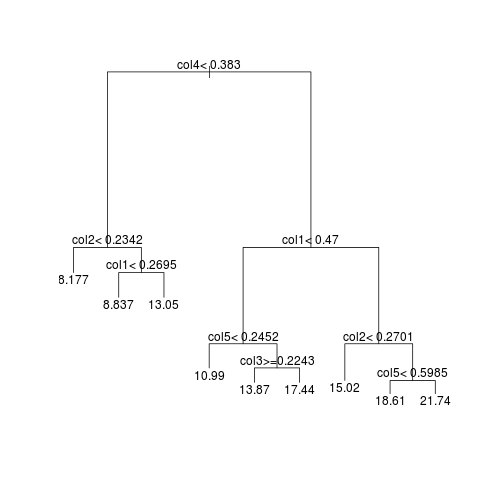
\includegraphics[totalheight=6cm]{./figs/tree_function.png}&
  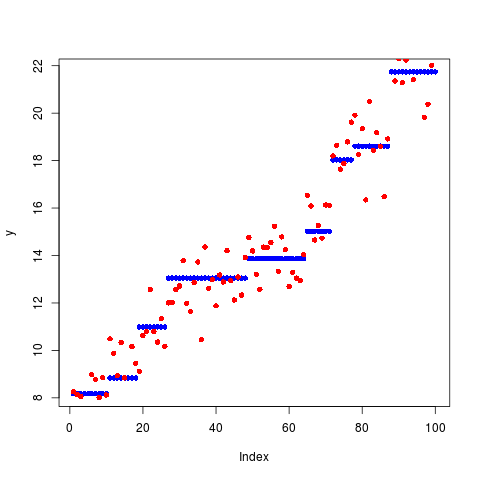
\includegraphics[totalheight=6cm]{./figs/noisy_tree_function.png}
 \end{tabular}
 \captionof{figure}{{\bf Synthetic data demonstrating RF's capability to cope with $p \gg n$.} {\bf a)} The tree
   function, where each split means XXXX. {\bf b)} A plot of the ordered $y$ variable for the tree example, and the $y$
   variable with added Gaussian noise (in red).}
  \label{figure:synth}
\end{figure}


\subsection*{CursedForest processes genome-wide variant data}
%\label{comp}
%Spark ML vs CursedForest vs Kmeans vs LR on small and full version (where applicable) of 1000G (performance and
%time/mem)

Traditionally, VariantSpark used the random forest algorithm from SparkML. While SparkML algorithms demonstrate
scalability when dealing with a large number of samples, this scalability quickly breaks down as we include more features.

One of the restrictions preventing SparkML algorithms from scaling to high-dimensionality data is the fact that the feature-set
for each individual is stored as a `Vector'. In Spark, Vectors are unable to be split and to process multiple vectors together,
the entirety of each vector must be loaded into memory on the same node. Therefore, as dimensionality increases, the
size of these Vectors must also increase, and subsequently this results in higher memory requirents.

On the other hand, CursedForest (CF) is specifically designed to handle wide ``cursed" data. It avoids the relation between
memory and dimensionality, by not using Vectors. Instead, CursedForest stores data in the Parquet columnar format.





\begin{table}[!ht]
\begin{adjustwidth}{-2.25in}{0in} % Comment out/remove adjustwidth environment if table fits in text column.
\caption{
{\bf Performance comparison between the different machine learning algorithms.}}
\begin{tabular}{|l+l|l|l|l|l|l|l|}
\hline
%\multicolumn{4}{|l|}{\bf Heading1} & \multicolumn{4}{|l|}{\bf Heading2}\\ \hline
\bf{Genome \%}  & \bf{method} & \bf{Accuracy} & \bf{Runtime} & \bf{Memory/Node} \\
\hline

\multirow{3}{*}{phase1\_chr22: 1,092 x 490,036} & CursedForest &  &  &  \\
& RF (Spark ML) &  &  &  \\
& RF (R) & 0.456 & 2.89 & 18GB \\ \hline

\multirow{3}{*}{phase3\_chr1: 2,504 x 6,450,364} & CursedForest & XX & 1hr 58min 23sec & 4GB \\
& RF (Spark ML) & 0.94 & 8hr 29min 07sec & 8GB \\
& LR &  & 10hr 30min & 8GB\\ \hline

\multirow{3}{*}{phase3\_chr1-3: 2,504 x 19,328,051}  & CursedForest & &  &\\
& RF(Spark ML) & &  &\\
& LR & &  &\\ \hline

\multirow{4}{*}{phase3\_chr1-22: 2,504 x 81,047,467} & CursedForest & 0.96 & 7hr 14min 40sec & 8GB \\ 
& RF (Spark ML) & - & - & - \\
& LR & - & - & - \\ 
& kmeans (Spark ML) & 0.82 & 30hr 44min 00sec & 24GB \\ \hline
\end{tabular}
\begin{flushleft} 
Comparison of different various machine learning libraries on different subsets of variant data 
from the 1000 Genomes Project. Size of the data is individuals x variants

\end{flushleft}
\label{table1}
\end{adjustwidth}
\end{table}


%\begin{table}
%\begin{minipage}{\textwidth}
%\begin{center}
%\begin{tabular}{|p{4.2cm}|l|l|l|l|l|l|l|}
%\hline
%\bf{method} & \bf{Accuracy} & \bf{Runtime} & \bf{Memory/Node} \\
%\hline
%RF (R)\footnote{10 nodes, 500 trees, dpas03} 
 %                                  &  0.456 & 2.89 & 18GB \\ \hline
%CursedForest\footnote{something}
 %                                  & X & X & X \\ \hline
%\end{tabular}
%\medskip
%\begin{flushleft} 
%\caption{Comparion between Random Forests on R and CursedForests on a smaller
%dataset. Chromosome 22 - phase1 (2.1GB) }
%\label{table:smaller_data}
%\end{flushleft}
%\end{center}
%\end{sidewaystable}
%\end{minipage}
%\end{table}




% \begin
% \begin{table}[!ht]
% \caption{
% {\bf Performance comparison between the different Machine Learning algorithms.}}
% \begin{tabular}{|p{4.2cm}|l|l|l|l|l|l|l|}
% \hline
% \bf{Genome }  & \bf{method} & \bf{Accuracy} & \bf{Runtime} & \bf{Memory/Node} \\
% \hline
%  chr 	 - phase1 (2.1GB)  &  RF (R) &  0.456 & 2.89 & 18GB \\ \hline
% \end{tabular}
% \begin{flushleft} 
% \end{flushleft}
% \label{table1}
% %\end{adjustwidth}
% \end{table}





\subsection*{Parameter settings}
We consider the parameter setting for the RF algorithm. We use the R terms from the package RandomForests
\cite{Liaw.and.Weiner.2002} which incoporates the original Fortran code by Brieman and Cutler. We incprporate the 
advice of \cite{Liaw.and.Weiner.2002}, which we have found mirrors our own experience.

\begin{itemize}
\item \texttt{ntree} the number of trees.  The number of trees necessary for good performance grows with the number of predictors.
  \marginpar{can we do proxmiity?}  \cite{Liaw.and.Weiner.2002} suggest that a high \texttt{ntree} is necessary to get stable
  estimates of variable importance and proximity; however, even though the variable importance measures may vary from run to run,
  the ranking of the importances is quite stable.  In addition, we note that it is possible for a RF model to have a very poor
  fit, and be useless for prediction, and still have a useful ranking of variable importance.
\item \texttt{mtry} --  the number of variables considered at each split (if \texttt{mtry}=$p$, we have a boosted decison
  tree model).  If one has a very large number of variables but expects only very few to be ``important'', using larger \texttt{mtry} may give
  better performance.
\item  For classification problems where the class frequencies are extremely unbalanced it may be necessary to change the prediction
  rule \marginpar{can we do this}
\item the size and complexity of the individual trees is controlled in RandomForests by setting \texttt{nodesize}, the
  minimum size of terminal nodes. It is controlled in Spark.ML by setting \texttt{maxDepth}, the maximum depth of each
  tree in the forest. The SparkML documentation somewhat unhelpfully sets \texttt{maxDepth=4} in their classification
  example\footnote{The documentation is available at \url{http://spark.apache.org/docs/latest/mllib-ensembles.html}.}.

  In the ATCG example the RandomForests code produced trees with depths of 30+. We note that Random forests are a way of averaging
  multiple deep decision trees, trained on different parts of the same training set, with the goal of reducing the
  variance. \url{https://en.wikipedia.org/wiki/Random_forest} and refs therein.  
\marginpar{are we including this  example?  Supplementary info?}
\end{itemize}


We note that it is possible for a RF model to have a very poor fit, and be useless for prediction, and still have a 
useful ranking of variable importance.


\begin{table}[!ht]
%\begin{adjustwidth}{-2.25in}{0in} % Comment out/remove adjustwidth environment if table fits in text column.
\caption{
{\bf Sensitivity analysis on parameter choice.}}
\begin{tabular}{|l|l|l|l|l|l|l|l|}
\hline
%\multicolumn{4}{|l|}{\bf Heading1} & \multicolumn{4}{|l|}{\bf Heading2}\\ \hline
\bf{Mtry}  & \bf{Mtree} & \bf{depth} & \bf{Accuracy} & \bf{Runtime} & \bf{Memory} \\
\hline
&&&&&\\ \hline
\end{tabular}
\begin{flushleft} 
  Table notes Phasellus venenatis, tortor nec vestibulum mattis, massa tortor interdum felis, nec pellentesque metus
  tortor nec nisl. Ut ornare mauris tellus, vel dapibus arcu suscipit sed.
\end{flushleft}
\label{table2}
%\end{adjustwidth}
\end{table}





%\subsection*{James' dataset}
%Comparing CursedForest with feature selection + linear model (performance and time/mem) 



\subsection*{Conclusion}



%\begin{table}[!ht]
%\begin{adjustwidth}{-2.25in}{0in} % Comment out/remove adjustwidth environment if table fits in text column.
%\caption{
%{\bf Table caption Nulla mi mi, venenatis sed ipsum varius, volutpat euismod diam.}}
%\begin{tabular}{|l|l|l|l|l|l|l|l|}
%\hline
%\multicolumn{4}{|l|}{\bf Heading1} & \multicolumn{4}{|l|}{\bf Heading2}\\ \hline
%$cell1 row1$ & cell2 row 1 & cell3 row 1 & cell4 row 1 & cell5 row 1 & cell6 row 1 & cell7 row 1 & cell8 row 1\\ \hline
%$cell1 row2$ & cell2 row 2 & cell3 row 2 & cell4 row 2 & cell5 row 2 & cell6 row 2 & cell7 row 2 & cell8 row 2\\ \hline
%$cell1 row3$ & cell2 row 3 & cell3 row 3 & cell4 row 3 & cell5 row 3 & cell6 row 3 & cell7 row 3 & cell8 row 3\\ \hline
%\end{tabular}
%\begin{flushleft} Table notes Phasellus venenatis, tortor nec vestibulum mattis, massa tortor interdum felis, nec pellentesque metus tortor nec nisl. Ut ornare mauris tellus, vel dapibus arcu suscipit sed.
%\end{flushleft}
%\label{table1}
%\end{adjustwidth}
%\end{table}


\section*{Supporting Information}

% Include only the SI item label in the subsection heading. Use the \nameref{label} command to cite SI items in the text.
\subsection*{S1 Video}
\label{S1_Video}
{\bf Bold the first sentence.}  Maecenas convallis mauris sit amet sem ultrices gravida. Etiam eget sapien nibh. Sed ac ipsum eget enim egestas ullamcorper nec euismod ligula. Curabitur fringilla pulvinar lectus consectetur pellentesque.

\subsection*{S1 Text}
\label{S1_Text}
{\bf Lorem Ipsum.} Maecenas convallis mauris sit amet sem ultrices gravida. Etiam eget sapien nibh. Sed ac ipsum eget enim egestas ullamcorper nec euismod ligula. Curabitur fringilla pulvinar lectus consectetur pellentesque.

\subsection*{S1 Table}
\label{S1_Table}
{\bf Lorem Ipsum.} Maecenas convallis mauris sit amet sem ultrices gravida. Etiam eget sapien nibh. Sed ac ipsum eget enim egestas ullamcorper nec euismod ligula. Curabitur fringilla pulvinar lectus consectetur pellentesque.

\section*{Acknowledgments}
Cras egestas velit mauris, eu mollis turpis pellentesque sit amet. Interdum et malesuada fames ac ante ipsum primis in faucibus. Nam id pretium nisi. Sed ac quam id nisi malesuada congue. Sed interdum aliquet augue, at pellentesque quam rhoncus vitae.

\nolinenumbers

%\section*{References}
% Either type in your references using
% \begin{thebibliography}{}
% \bibitem{}
% Text
% \end{thebibliography}
%
% OR
%
% Compile your BiBTeX database using our plos2015.bst
% style file and paste the contents of your .bbl file
% here.
% 

\bibliography{./CursedForest.bib}

\end{document}





  \item D\iaz-Uriarte, R., \& Alvarez de Andr\es, S. (2006). Gene selection and classification of microarray data using random
    forest. BMC Bioinformatics, 7, 3. http://doi.org/10.1186/1471-2105-7-3
  \item Goldstein, B. A., Polley, E. C., & Briggs, F. B. S. (2011). Random Forests for Genetic Association Studies. Statistical
    Applications in Genetics and Molecular Biology, 10(1), 32. http://doi.org/10.2202/1544-6115.1691



@article{Chen2012323,
title = "Random forests for genomic data analysis ",
journal = "Genomics ",
volume = "99",
number = "6",
pages = "323 - 329",
year = "2012",
note = "",
issn = "0888-7543",
doi = "http://dx.doi.org/10.1016/j.ygeno.2012.04.003",
url = "http://www.sciencedirect.com/science/article/pii/S0888754312000626",
author = "Xi Chen and Hemant Ishwaran",
keywords = "Random forests",
keywords = "Random survival forests",
keywords = "Classification",
keywords = "Prediction",
keywords = "Variable selection",
keywords = "Genomic data analysis ",
abstract = "Random forests (RF) is a popular tree-based ensemble machine learning tool that is highly data adaptive, applies to “large p, small n” problems, and is able to account for correlation as well as interactions among features. This makes \{RF\} particularly appealing for high-dimensional genomic data analysis. In this article, we systematically review the applications and recent progresses of \{RF\} for genomic data, including prediction and classification, variable selection, pathway analysis, genetic association and epistasis detection, and unsupervised learning. "
}